
\section{The Electric Potential\footnote{%
1990-93 Dept. of Physics and Astronomy, Dickinson College. Supported
by FIPSE (U.S. Dept. of Ed.) and NSF. Portions of this material may
have been modified locally and may not have been classroom tested
at Dickinson College.
}}

Name \rule{2.0in}{0.1pt}\hfill{}Section \rule{1.0in}{0.1pt}\hfill{}Date
\rule{1.0in}{0.1pt}

\textbf{Overview}

It takes work to lift an object in the earth's gravitational field.
Lowering the object releases the energy that was stored as potential
energy when it was lifted. Last semester, we applied the term \emph{conservative}
to the gravitational force because it {}``releases'' \underbar{all}
of the stored energy. We found experimentally that the work required
to move a mass in the gravitational field was path independent. This
is an important property of any conservative force. Given the mathematical
similarity between the Coulomb force and the gravitational force,
it should come as no surprise that experiments confirm that an electric
field is also conservative. This means that the work needed to move
a charge from point A to point B is independent of the path taken
between points. A charge could be moved directly between the two points
or looped around and the work expended to take either path would be
the same. Work done by an electric field on a test charge q traveling
between points A and B is given by

{\centering \( W=\int ^{B}_{A} \)\( \overrightarrow{F}\cdot d\overrightarrow{s}=\int ^{B}_{A}q\overrightarrow{E}\cdot d\overrightarrow{s} \)\par}

\textbf{Activity 1: Work Done on a Charge Traveling in a Uniform Electric
Field}

(a) A charge q travels a distance d from point A to point B; the path
is parallel to a uniform electric field of magnitude E. What is the
work done by the field on the charge? How does the form of this equation
compare to the work done on a mass m traveling a distance d in the
almost uniform gravitational field near the surface of the earth?

\vspace{0.3cm}
{\centering \resizebox*{0.2\textwidth}{!}{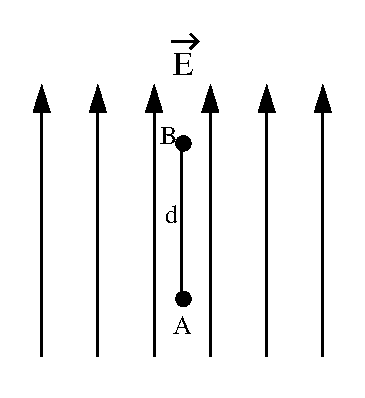
\includegraphics{electric_potential_fig_1.eps}} \par}
\vspace{0.3cm}

(b) The charge $q$ travels a distance $d$ from point $A$ to point $B$ in a
uniform electric field of magnitude $E$, but this time the path is perpendicular
to the field lines. What is the work done by the field on the charge?

\vspace{0.3cm}
{\centering \resizebox*{0.2\textwidth}{!}{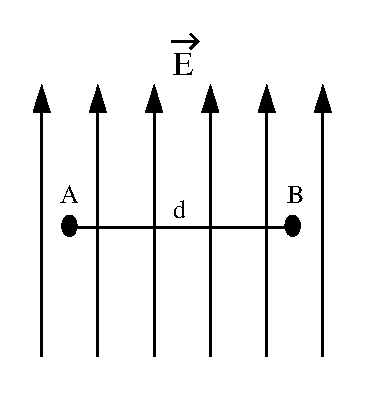
\includegraphics{electric_potential_fig_2.eps}} \par}
\vspace{0.3cm}

(c) The charge $q$ travels a distance $d$ from point $A$ to point $B$ in a
uniform electric field of magnitude $E$. The path lies at a 45\( ^{\circ } \)
angle to the field lines. What is the work done by the field on the
charge?
\vspace{10mm}

\vspace{0.3cm}
{\centering \resizebox*{0.2\textwidth}{!}{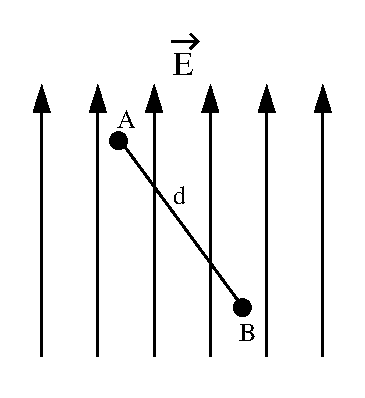
\includegraphics{electric_potential_fig_3.eps}} \par}
\vspace{0.3cm}

\textbf{Potential Energy and Potential Difference}

Recall that by definition the work done by a conservative force equals
the negative of the change in potential energy, so that the change
in potential energy of a charge moving from point $A$ to point $B$ under
the influence of an electrical force is given by:

{\centering \( \Delta U=U_{B}-U_{A}=-\int ^{B}_{A}q\overrightarrow{E}\cdot d\overrightarrow{s} \)\par}

By analogy to the definition of the electric field, we are interested
in defining the \emph{electric potential difference} \( \Delta V=V_{B}-V_{A} \)
as the change in electric potential energy \( \Delta U \) per
unit charge. Formally, \emph{the potential difference is defined as
the work per unit charge that an external agent must perform to move
a test charge from A to B without changing its kinetic energy}. The
potential difference has units of joules per coulomb. Since 1 J/C
is defined as one \emph{volt}, the potential difference is often referred
to as \emph{voltage}.

\textbf{Activity 2: The Equation for Potential Difference}

Write the equation for potential difference as a function of \( \overrightarrow{E} \),
\( d\overrightarrow{s} \), $A$, and $B$.
\vspace{15mm}

\textbf{The Potential Difference for a Point Charge}

The simplest charge configuration that can be used to consider how
voltage changes between two points in space is a single point charge.
We will start by considering a single point charge and then move on
to more complicated configurations of charge.

A point charge $q$ produces an electric field that points radially outward
in all directions for a positive charge, radially inward for a negative charge. The line integral equation for the potential difference
can be evaluated to find the potential difference between any two
points in space $A$ and $B$ (a line integral is one that follows a path
through space).

It is common to choose the reference point for the determination of
voltage to be set at infinity so that we are determining the work
per unit charge that is required to bring a test charge from infinity
to a certain point in space. Let's choose a coordinate system so that
the point charge is conveniently located at the origin. In this case
we will be interested in the potential difference between infinity
and some point which is a distance r from the point charge. Thus,
we can write the equation for the potential difference, or voltage,
as

{\centering \( \Delta V=V_{B}-V_{A}=V_{r}-V_{\infty }=-\int ^{r}_{\infty }\overrightarrow{E}\cdot d\overrightarrow{s} \)\par}

Often, when the reference point for the potential difference is at
infinity, this difference is simply referred to as {}``the potential'',
and the symbol \( \Delta V \) is just replaced with the symbol $V$.

\textbf{Activity 3: Potential at a Distance r from a Charge}

Starting from the expression for the electric field of a point charge,
show that, if $A$ is at infinity and $B$ is a distance $r$ from a point
charge $q$, then the potential $V$ is given by the expression

{\centering \( V=\frac{kq}{r} \)\par}

where \( k=\frac{1}{4\pi \varepsilon _{\circ }} \)= 8.99 x 10\( ^{9} \)
Nm\( ^{2} \)/ C\( ^{2} \).

\vspace{0.3cm}
{\centering \resizebox*{0.4\textwidth}{!}{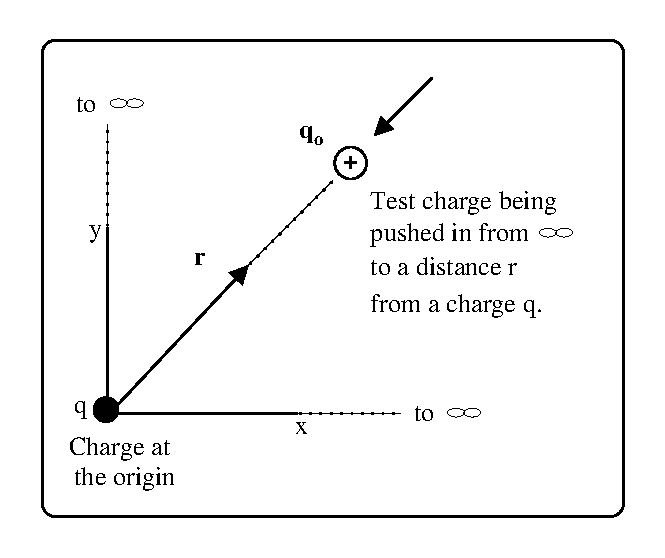
\includegraphics{electric_potential_fig_4.eps}} \par}
\vspace{0.3cm}

\textbf{Hint:} What is the mathematical expression for an $E$-field
from a point charge?
\vspace{30mm}

\textbf{Activities 4 and 5: Potential Due to Continuous Charge Distributions}

The potential from a continuous charge distribution can be calculated
several ways. Each method should yield approximately the same result.
First, we can use an integral method in which the potential $dV$ from
each element of charge $dq$ is integrated mathematically to give a total
potential at the location of interest. Second, we can approximate
the value of the potential $V$ by summing up several finite elements
of charge \( \Delta q \) by using a computer spreadsheet or hand
calculations.

Again, let's consider a relatively simple charge distribution. In
this case we will look at a ring with charge uniformly distributed
on it. We will calculate the potential on the axis passing through
the center of the ring as shown in the diagram below. (Later on you
could find the potential difference from a disk or a sheet of charge
by considering a collection of nested rings).

\vspace{0.3cm}
{\centering 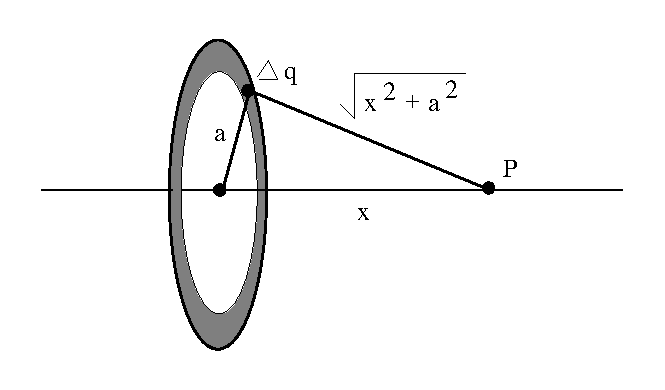
\includegraphics{electric_potential_fig_5.eps} \par}
\vspace{0.3cm}

\vspace{2in}
A ring of charge has a total charge of $Q = 20$\( \mu  \)C (i.e. 20
x 10\( ^{-6} \) C). The radius of the ring, $a$, is 30 cm. We want
to find the electric field and the electric potential at a distance $x$ from the ring along an axis that is perpendicular to the ring
and passes through its center. Let's begin by calculating the potential
in the next activity.

\textbf{Hints:} Since the potential is a scalar and not a vector we
can calculate the potential at point $P$ (relative to \( \infty  \))
for each of the charge elements \( \Delta q \) and add them to each
other. This looks like a big deal but it is actually a trivial problem
because all the charge elements are the same distance from point $P$.

\textbf{Activity 4: Numerical Estimate of the Potential due to a Charged
Ring}

(a) Divide the ring into 20 elements, each of charge \( \Delta q \) = 1.0 x 10\( ^{-6} \) C and
calculate the total $V$ at a distance of $x$ = 20 cm from the center of
the ring using a spreadsheet program or by hand calculation. Summarize
the result below. Be sure to attach a printout of your spreadsheet
results.
\vspace{1.5in}

\textbf{Activity 5: Calculation of the Potential due to a Charged Ring}

By following the steps below, you can use an integral to find a more
exact value of the potential.

(a) Show that

{\centering \( V=k\int \frac{dq}{r}=k\int \frac{dq}{\sqrt{x^{2}+a^{2}}} \)\par}
\vspace{25mm}

(b) Explain why

{\centering \( k\int \frac{dq}{\sqrt{x^{2}+a^{2}}}=\frac{k}{\sqrt{x^{2}+a^{2}}}\int dq \)\par}

(i.e. explain why \( \sqrt{x^{2}+a^{2}} \) can be pulled out of the integral).
\vspace{20mm}

(c) Perform the integration in part (b) above. Then substitute values
for $a$, $x$, and $Q$ into the resulting expression in order to obtain a
more {}``exact'' value for the potential.
\vspace{25mm}

(d) How does the {}``numerical'' value that you obtained in Activity
4 compare with the {}``exact'' value you obtained in (c)?
\vspace{20mm}

Now let's take a completely different approach to the same problem.
If we can find the vector equation for the electric field at point
P due to the ring of charge, then we can use the expression

{\centering \( \Delta V=V_{r}-V_{\infty }=-\int ^{r}_{\infty }\overrightarrow{E}\cdot d\overrightarrow{s} \)\par}

as an alternative way to find a general equation for the potential
at point $P$.

\vspace{0.3cm}
{\centering 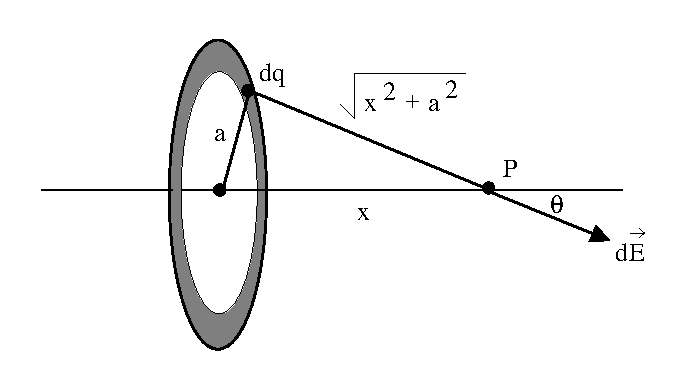
\includegraphics{electric_potential_fig_6.eps} \par}
\vspace{0.3cm}

\textbf{Activity 6: \( \Delta  \)V from a Ring Using the E-field
Method}

(a) Starting from the electric field of a point charge, show that
the electric field at point P from the charged ring is given by

{\centering \( \overrightarrow{E}=\frac{kqx}{(x^{2}+a^{2})^{3/2}}\hat{x} \)\par}

\textbf{Hints:} (1) Why is there no y component of the E-field? (2)
\( \cos \theta =\frac{x}{\sqrt{x^{2}+a^{2}}} \)
\vspace{30mm}

(b) To find \( \Delta  \)V use the following equation.

{\centering \( \Delta V=V_{r}-V_{\infty }=-\int ^{r}_{\infty }\overrightarrow{E}\cdot d\overrightarrow{s} \)\par}
\textbf{Hint:} You will probably need to consult the integral tables in the appendix of your text.
\textbf{Note:} The above expression for \overrightarrow{E} is only valid along the $x$-axis.
\vspace{30mm}

(c) How does the result compare to that obtained in Activity 5 (c)?
\vspace{30mm}

\textbf{Equipotential Surfaces}

Sometimes it is possible to move along a surface without doing any
work. Thus, it is possible to remain at the same potential energy
anywhere along such a surface. If an electric charge can travel along
a surface without doing any work, the surface is called an \emph{equipotential
surface}.

Consider the three different charge configurations shown below. Where
are the equipotential surfaces? What shapes do they have?

\textbf{Hint:} If you have any computer simulations available to you
for drawing equipotential lines associated with electrical charges,
you may want to check your guesses against the patterns drawn in one
or more of the simulations.

\textbf{Activity 7: Sketches of Electric Field Lines and Equipotentials}

(a) Suppose that you are a test charge and you start moving at some
distance from the charge below (such as 4 cm). What path could you
move along without doing any work, i.e. \( \overrightarrow{E}\cdot d\overrightarrow{s} \)
is always zero? What is the shape of the equipotential surface? Remember
that in general you can move in \emph{three} dimensions.

\vspace{0.3cm}
{\centering \resizebox*{0.3\columnwidth}{!}{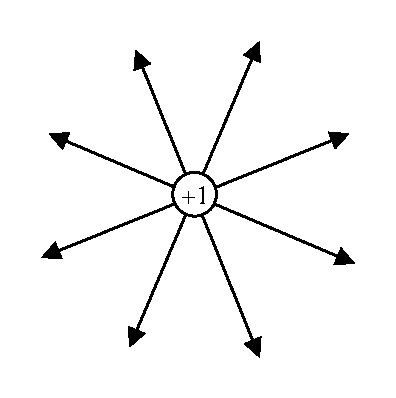
\includegraphics{electric_potential_fig_7.eps}} \par}
\vspace{0.3cm}

(b) Find some equipotential surfaces for the charge configuration
shown below, which consists of two charged metal plates placed parallel
to each other. What is the shape of the equipotential surfaces?

\vspace{0.3cm}
{\centering \resizebox*{0.28\textwidth}{!}{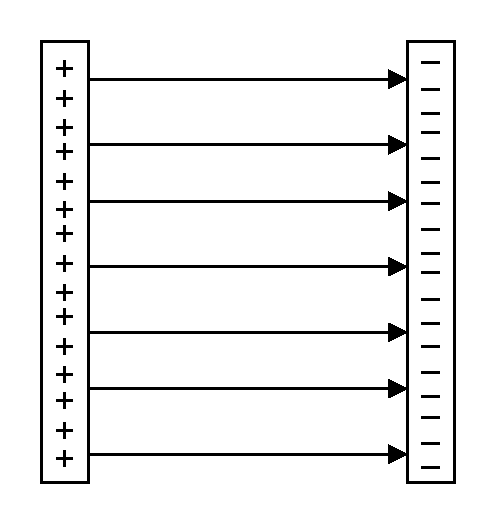
\includegraphics{electric_potential_fig_8.eps}} \par}
\vspace{0.3cm}

(c) Find some equipotential surfaces for the electric dipole charge
configuration shown below.

\vspace{0.3cm}
{\centering \resizebox*{0.25\textwidth}{!}{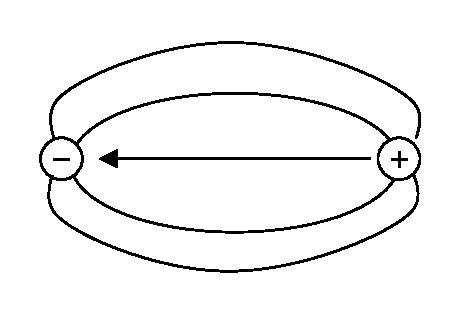
\includegraphics{electric_potential_fig_9.eps}} \par}
\vspace{0.3cm}

(d) In general, what is the relationship between the direction of
the equipotential lines you have drawn (representing that part of
the equipotential surface that lies in the plane of the paper) and
the direction of the electric field lines?\vspace{15mm}

